\documentclass[11pt,a4paper]{article}

\usepackage[utf8]{inputenc}
\usepackage[T1]{fontenc}
\IfFileExists{lmodern.sty}{\usepackage{lmodern}}{}
\usepackage[margin=2.4cm]{geometry}
\usepackage{amsmath,amssymb,bm}
\usepackage{siunitx}
\usepackage{booktabs}
\usepackage{tikz}
\usetikzlibrary{arrows.meta,calc,decorations.pathmorphing}
\usepackage{enumitem}
\usepackage[colorlinks=true,linkcolor=blue!50!black,citecolor=green!40!black,urlcolor=blue!60!black]{hyperref}

\sisetup{separate-uncertainty=true,range-phrase=--}

\newcommand{\ee}{\mathrm{e}}
\newcommand{\ii}{\mathrm{i}}
\newcommand{\dd}{\mathrm{d}}
\newcommand{\kB}{k_\mathrm{B}}
\newcommand{\ER}{E_\mathrm{R}}
\newcommand{\Ulat}{U_\mathrm{lat}}
\newcommand{\Voff}{V_\mathrm{off}}
\newcommand{\Neff}{N_\mathrm{eff}}
\newcommand{\vperp}{\bm{v}_\perp}
\newcommand{\rperp}{\bm{r}_\perp}

\title{Ultracold $^{87}$Rb in a vertical 1064\,nm standing wave above a hollow-core fiber:\\
physics background and simulation method\\[4pt]
\large Semiclassical DSMC with band-resolved collisions}
\author{Project notes --- \texttt{rb\_lattice\_dsmc}}
\date{Version 1, 23 October 2026}

\begin{document}
\maketitle

\begin{abstract}
These notes collect the physics needed to understand, implement and critically assess a direct-simulation Monte Carlo (DSMC) model of ultracold $^{87}$Rb atoms ($T=1$--$\SI{5}{\micro K}$) held in a vertical, nearly counter-propagating \SI{1064}{nm} standing wave whose beams are focused on the output facet of a hollow-core fiber (HCF). We review the optical dipole potential, the geometry of the two-beam field (wavefront curvature, Gouy phase, small crossing angle), band structure in a tilted 1D lattice, quasi-two-dimensional collisions and Bird's DSMC algorithm. We then describe the semiclassical model adopted here --- quantized axial motion (band index), classical radial motion, band-resolved golden-rule collisions --- together with the treatment of losses, of atoms falling into the fiber, and the definition of all observables stored by the simulation. The text is written for a PhD student in AMO physics; key references are given for each topic.
\end{abstract}

\tableofcontents
\newpage

%=======================================================================
\section{Overview of the problem}
\label{sec:overview}
%=======================================================================

Cold atoms from an optical molasses are captured in a 1D optical lattice formed by two red-detuned beams at $\lambda=\SI{1064}{nm}$ (Fig.~\ref{fig:geometry}). Beam~1 exits a hollow-core fiber whose facet defines $z=0$ and propagates upward ($+z$); beam~2 propagates downward, tilted by a small angle $\theta=10^{-4}$--$10^{-2}$\,rad. Both beams have a waist $w_0=\SI{20}{\micro m}$ located at the facet, and their axes cross there. The atom cloud (diameter \SI{2}{mm} along $z$) is centred at $z_c=5$--\SI{8}{mm}, far beyond the Rayleigh range $z_R=\pi w_0^2/\lambda=\SI{1.18}{mm}$. Gravity points toward the fiber.

The questions the simulation must answer are: how many atoms stay trapped over $\sim\SI{200}{ms}$, through which channels the others are lost (radially, or by falling down the lattice onto/into the fiber), how the energy is distributed between kinetic and potential, axial and radial degrees of freedom, and how all this depends on two-body collisions. Table~\ref{tab:scales} anticipates the main scales; the rest of these notes explains where they come from.

\begin{figure}[t]
\centering
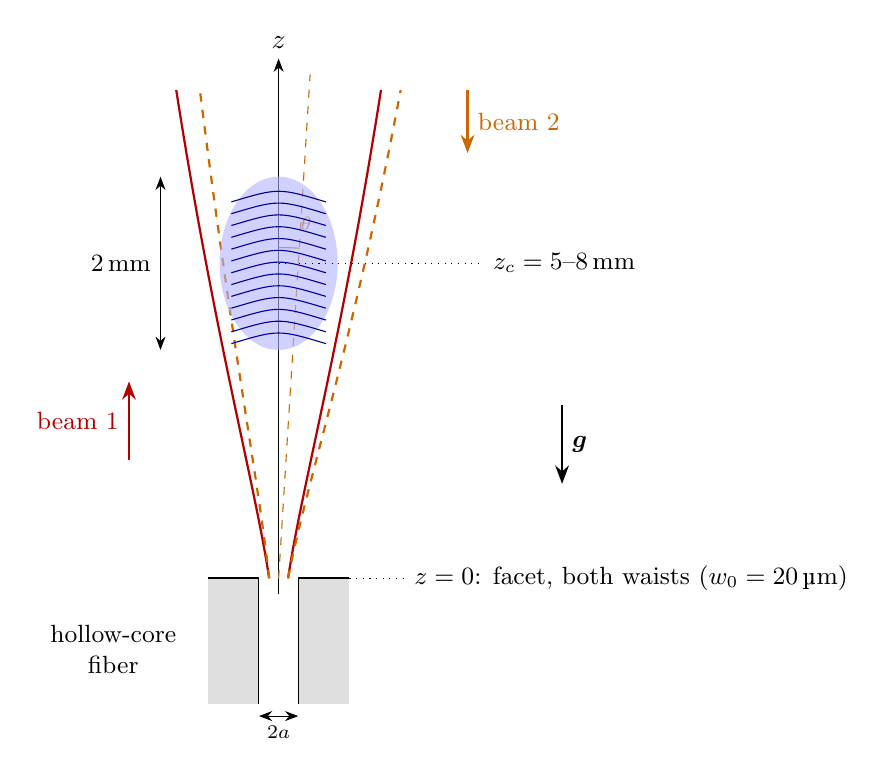
\begin{tikzpicture}[scale=1.0,>=Stealth]
  % fiber
  \fill[gray!25] (-0.9,-1.6) rectangle (-0.25,0);
  \fill[gray!25] (0.25,-1.6) rectangle (0.9,0);
  \fill[white] (-0.25,-1.6) rectangle (0.25,0);
  \draw[thick] (-0.9,0) -- (-0.25,0) (0.25,0) -- (0.9,0);
  \draw (-0.25,-1.6) -- (-0.25,0) (0.25,-1.6) -- (0.25,0);
  \node[align=center,font=\small] at (-2.1,-0.9) {hollow-core\\fiber};
  \draw[<->] (-0.25,-1.75) -- (0.25,-1.75) node[midway,below,font=\scriptsize] {$2a$};
  % beam envelopes (beam 1, vertical)
  \draw[red!70!black,thick] (0.12,0) .. controls (0.3,1.2) and (0.8,3) .. (1.3,6.2);
  \draw[red!70!black,thick] (-0.12,0) .. controls (-0.3,1.2) and (-0.8,3) .. (-1.3,6.2);
  % beam 2 (slightly tilted)
  \draw[orange!80!black,thick,dashed] (0.12,0) .. controls (0.35,1.2) and (0.95,3) .. (1.55,6.2);
  \draw[orange!80!black,thick,dashed] (-0.12,0) .. controls (-0.25,1.2) and (-0.6,3) .. (-1.0,6.2);
  % axes
  \draw[->] (0,-0.2) -- (0,6.6) node[above] {$z$};
  \draw[orange!80!black,dashed] (0,0) -- (0.4,6.4);
  \draw[orange!80!black] (0,4.2) arc (90:86.4:4.2);
  \node[orange!80!black,font=\scriptsize] at (0.35,4.5) {$\theta$};
  % cloud
  \fill[blue!30,opacity=0.6] (0,4.0) ellipse (0.75 and 1.1);
  \foreach \y in {3.1,3.25,...,4.95} {\draw[blue!60!black,thin] (-0.6,\y-0.12) .. controls (0,\y+0.06) .. (0.6,\y-0.12);}
  \draw[<->] (-1.5,2.9) -- (-1.5,5.1) node[midway,left,font=\small] {\SI{2}{mm}};
  \draw[dotted] (0,4.0) -- (2.6,4.0) node[right,font=\small] {$z_c=5$--\SI{8}{mm}};
  % arrows of propagation
  \draw[->,red!70!black,thick] (-1.9,1.5) -- (-1.9,2.5) node[midway,left,font=\small] {beam 1};
  \draw[->,orange!80!black,thick] (2.4,6.2) -- (2.4,5.4) node[midway,right,font=\small] {beam 2};
  \draw[->,thick] (3.6,2.2) -- (3.6,1.2) node[midway,right,font=\small] {$\bm g$};
  \draw[dotted] (0.9,0) -- (1.6,0) node[right,font=\small] {$z=0$: facet, both waists ($w_0=\SI{20}{\micro m}$)};
\end{tikzpicture}
\caption{Geometry (not to scale). The lattice planes inside the cloud are curved (radius $\simeq z$) because both beams diverge from the same focus at the facet.}
\label{fig:geometry}
\end{figure}

%=======================================================================
\section{Atom--light interaction: the optical dipole potential}
\label{sec:dipole}
%=======================================================================

\subsection{Dipole potential and scattering rate}

For a far-detuned field $\bm E(\bm r,t)=\mathrm{Re}[\bm{\mathcal E}(\bm r)\ee^{-\ii\omega t}]$ the ground-state light shift is
\begin{equation}
U(\bm r) = -\frac{1}{4}\,\mathrm{Re}\,\alpha(\omega)\,|\bm{\mathcal E}(\bm r)|^2
         = -\frac{\mathrm{Re}\,\alpha(\omega)}{2\varepsilon_0 c}\, I(\bm r),
\qquad I=\tfrac12\varepsilon_0 c|\bm{\mathcal E}|^2 ,
\label{eq:Udip}
\end{equation}
and the photon scattering rate is $\Gamma_\mathrm{sc}=\mathrm{Im}\,\alpha\, I/(\hbar\varepsilon_0 c)$~\cite{Grimm2000}. For alkali atoms at \SI{1064}{nm} both D lines contribute; the multilevel expression (including counter-rotating terms) is given in Ref.~\cite{Grimm2000}. With linear polarization the vector light shift vanishes and the potential is the same for all hyperfine Zeeman states (the tensor part is negligible for the $5S_{1/2}$ ground state). We use the scalar dynamic polarizability $\alpha(\SI{1064}{nm})\simeq 687\,$a.u.~\cite{Safronova2006}, with $\alpha_\mathrm{SI}=4\pi\varepsilon_0 a_0^3\,\alpha_\mathrm{a.u.}$. Atoms are attracted to intensity maxima.

A useful rule of thumb is $\Gamma_\mathrm{sc}\approx |U|\,\Gamma/(\hbar|\Delta_\mathrm{eff}|)$; for the deepest lattice considered ($|U|\simeq\SI{40}{\micro K}$) this gives $\Gamma_\mathrm{sc}\lesssim\SI{0.3}{s^{-1}}$, i.e.\ fewer than 0.06 photons per atom in \SI{200}{ms}. Photon recoil heating in a lattice (band-changing Raman processes in the Lamb--Dicke regime) is analysed in Ref.~\cite{Gerbier2010}; it is an optional, small effect here.

\subsection{Atomic data}
\begin{center}
\begin{tabular}{@{}lll@{}}
\toprule
mass & $m=86.909\,$u & \cite{Steck87}\\
$s$-wave scattering length, $|F{=}1,m_F{=}{-}1\rangle$ & $a=100.4\,a_0$ & \cite{vanKempen2002}\\
polarizability at \SI{1064}{nm} & $\alpha\simeq 687\,$a.u. & \cite{Safronova2006}\\
recoil energy at \SI{1064}{nm} & $\ER=\hbar^2k^2/2m=h\times\SI{2.03}{kHz}=\kB\times\SI{97}{nK}$ & \\
three-body loss (thermal) & $K_3\approx 4\times10^{-29}\,\mathrm{cm^6\,s^{-1}}$ & \cite{Burt1997}\\
\bottomrule
\end{tabular}
\end{center}

%=======================================================================
\section{Geometry of the two-beam field}
\label{sec:geometry}
%=======================================================================

\subsection{Gaussian beams}
A TEM$_{00}$ beam propagating along $+s$ with waist $w_0$ at $s=0$ has~\cite{Siegman}
\begin{equation}
\mathcal E(\rho,s) = \mathcal E_0\frac{w_0}{w(s)}\exp\!\left[-\frac{\rho^2}{w(s)^2}\right]
\exp\!\left[-\ii\left(ks+\frac{k\rho^2}{2R(s)}-\zeta(s)\right)\right],
\label{eq:gauss}
\end{equation}
\begin{equation}
w(s)=w_0\sqrt{1+s^2/z_R^2},\qquad R(s)=s\left(1+z_R^2/s^2\right),\qquad \zeta(s)=\arctan(s/z_R),
\end{equation}
with $I(\rho,s)=\frac{2P}{\pi w(s)^2}\ee^{-2\rho^2/w(s)^2}$. The expressions are valid for negative $s$ (before the focus) with $R$ and $\zeta$ odd functions of $s$. For $z_c=5$--\SI{8}{mm} we are in the far field: $w\simeq w_0 z/z_R=87$--\SI{137}{\micro m}, $R\simeq z$.

\subsection{Interference of the two beams}
Let beam~1 propagate along $+z$ (axis $\hat{\bm z}$ through the origin) and beam~2 along $-\hat{\bm e}_2$, with $\hat{\bm e}_2=(\sin\theta,0,\cos\theta)$, also through the origin. Beam~2 is converging toward the facet: its own propagation coordinate is $s_2=-\bm r\cdot\hat{\bm e}_2<0$ and its transverse distance is $\rho_2^2=r^2-(\bm r\cdot\hat{\bm e}_2)^2$. Writing $\mathcal E_i=A_i\ee^{-\ii\varphi_i}$ and assuming parallel linear polarizations, the total intensity is
\begin{equation}
I = I_1+I_2+2\sqrt{I_1I_2}\cos\Phi,\qquad \Phi(\bm r)=\varphi_1(\bm r)-\varphi_2(\bm r)+\phi_0 ,
\end{equation}
where $\phi_0$ is a constant (path-length) phase that merely translates the lattice. On the common axis ($\theta=0$),
\begin{equation}
\Phi \simeq 2kz+\frac{k\rho^2}{R(z)}-2\zeta(z).
\label{eq:Phi}
\end{equation}
Three consequences are important:
\begin{enumerate}[leftmargin=*]
\item \textbf{Lattice spacing.} $|\nabla\Phi|\simeq 2k$, so the period is $d=\lambda/2=\SI{532}{nm}$. The Gouy term changes the local period by a relative amount $\sim z_R/(k z^2)\sim10^{-5}$: negligible, but included automatically if $\Phi$ is computed exactly.
\item \textbf{Curved planes.} Surfaces of constant $\Phi$ are $z\simeq z_j-\rho^2/(2R)$: domes of radius $R\simeq z$. Across one beam radius the plane bends by $w^2/2R\simeq\SI{0.7}{\micro m}>d$. A product ansatz ``Gaussian envelope $\times\cos^2 kz$'' is therefore \emph{wrong} for radial motion; the site surfaces must be followed.
\item \textbf{Crossing angle.} For small $\theta$, $s_2\simeq-(z+\theta x)$ and $\rho_2^2\simeq(x-\theta z)^2+y^2$. The planes tilt by $\theta/2$ and the axis of beam~2 is displaced by $\theta z$ (\SI{0.5}{\micro m} for $\theta=10^{-4}$, up to \SI{80}{\micro m} for $\theta=10^{-2}$). The intensity product $\sqrt{I_1I_2}$, which sets the lattice modulation, is maximal on the bisector $x=\theta z/2$ and reduced by $\exp[-(\theta z)^2/(2w^2)]$ there (0.84 at $\theta=10^{-2}$, $z=\SI{7}{mm}$).
\end{enumerate}

\subsection{Lattice depth, offset, and site surfaces}
With $U_i=\alpha I_i/(2\varepsilon_0c)$ the potential including gravity is
\begin{equation}
V(\bm r) = -U_1-U_2-2\sqrt{U_1U_2}\cos\Phi + mgz
= \Voff(\bm r) - \Ulat(\bm r)\cos^2\!\frac{\Phi}{2} + mgz,
\label{eq:Vfull}
\end{equation}
\begin{equation}
\Ulat=4\sqrt{U_1U_2},\qquad \Voff=-\left(\sqrt{U_1}-\sqrt{U_2}\right)^2 .
\end{equation}
For balanced, perfectly overlapped beams $\Voff=0$ and $\Ulat=4U_1$ (a factor 4 deeper than a single beam). Imbalance or displacement produces a non-modulated (running-wave) offset $\Voff<0$. Sites (antinodes) are the surfaces $\Phi(\bm r)=2\pi j$, $j\in\mathbb Z$; we parametrize site $j$ by its height $z_j(x,y)$, obtained by Newton iteration on $\Phi(x,y,z)=2\pi j$ starting from $z_j(0,0)\simeq jd$.

The gravitational energy per site is $mgd=\kB\times\SI{55}{nK}$, far below $\Ulat=6$--\SI{42}{\micro K}: each site is an independent well, and gravity only matters (i) as a small tilt of the 1D lattice (Sec.~\ref{sec:tilt}), (ii) along the curved site surface, where $mg z_j(\rho)\simeq -mg\rho^2/2R$ is a weak radial anti-confinement (it reduces $\omega_r^2$ by $g/R$, a $\lesssim2\%$ effect), and (iii) for atoms that are no longer bound to a site.

%=======================================================================
\section{Atoms in a tilted 1D lattice}
\label{sec:lattice}
%=======================================================================

\subsection{Band structure: the Mathieu problem}
Locally, along the normal to the site surfaces (coordinate $\xi\simeq z$), the potential is $-\Ulat\cos^2(k\xi)$ (we drop the slowly varying $\Voff$). With $x=k\xi$ and $s\equiv\Ulat/\ER$ the Schrödinger equation becomes Mathieu's equation~\cite{DLMF28,Morsch2006}
\begin{equation}
\psi''(x)+\left[a-2q\cos 2x\right]\psi(x)=0,\qquad q=\frac{s}{4},\qquad E=\ER\, a-\frac{\Ulat}{2},
\end{equation}
(after the shift $x\to x+\pi/2$). Band $n=0,1,\dots$ spans $E\in[\ER a_n(q)-\Ulat/2,\ \ER b_{n+1}(q)-\Ulat/2]$, where $a_n,b_n$ are the Mathieu characteristic values (available in \texttt{scipy.special}). The gap between bands $n$ and $n+1$ is $\Delta_n=\ER[a_{n+1}(q)-b_{n+1}(q)]$. In the deep-lattice limit
\begin{equation}
E_n\simeq-\Ulat+\hbar\omega_z\left(n+\tfrac12\right)-\frac{\ER}{4}\left(2n^2+2n+1\right),\qquad
\hbar\omega_z=2\sqrt{s}\,\ER ,
\label{eq:anharm}
\end{equation}
and the lowest Wannier functions are close to harmonic-oscillator states of width $l_z=\sqrt{\hbar/m\omega_z}=k^{-1}s^{-1/4}$. For our parameters $s=65$--$430$, $\hbar\omega_z/\kB=1.6$--\SI{4}{\micro K}, $l_z\simeq30$--\SI{45}{nm} and only 5--13 bands lie below the barrier. Because $\hbar\omega_z\sim\kB T$, the axial motion cannot be treated classically: this is the reason for the semiclassical model of Sec.~\ref{sec:semiclassical}. The Lamb--Dicke parameter $\eta_\mathrm{LD}=k l_z/\sqrt2=s^{-1/4}/\sqrt2\approx0.16$--$0.25$.

Two quantities derived from the bands are needed below. By the Hellmann--Feynman theorem, the mean lattice potential energy and kinetic energy in band $n$ are
\begin{equation}
\langle V_\mathrm{lat}\rangle_n=\Ulat\frac{\partial E_n}{\partial \Ulat}=s\frac{\dd E_n}{\dd s},\qquad
\langle T_z\rangle_n=E_n-\langle V_\mathrm{lat}\rangle_n ,
\label{eq:HF}
\end{equation}
and $\partial E_n/\partial\Ulat=-\langle\cos^2 k\xi\rangle_n\in(-1,0)$: atoms in higher bands are less strongly attracted toward regions of larger $\Ulat$.

\subsection{Tilted lattice: Bloch oscillations, Wannier--Stark states and Landau--Zener tunnelling}
\label{sec:tilt}
Gravity adds a linear potential $F\xi$ with $F=mg$. In a tilted lattice the quasimomentum evolves as $\hbar\dot q=-F$, so atoms undergo Bloch oscillations at $\nu_B=Fd/h=\SI{1.14}{kHz}$~\cite{BenDahan1996}. Equivalently the eigenstates are Wannier--Stark ladders spaced by $Fd$ and localized over $W_n/Fd$ sites, $W_n$ being the band width~\cite{Gluck2002}. For deep bands $W_n\ll Fd$ and atoms are localized on a single site; for the topmost bound bands $W_n\sim0.2$--\SI{0.7}{\micro K} and the Bloch-oscillation amplitude spans a few to $\sim10$ sites, which does not cause loss.

Loss along the lattice requires interband (Landau--Zener) tunnelling to the continuum. In the weak-binding form, the probability per Bloch period of crossing gap $\Delta_n$ is~\cite{Peik1997}
\begin{equation}
P_\mathrm{LZ}=\exp\!\left(-\frac{\pi\Delta_n^2}{4\hbar^2 k\,g}\right),\qquad \Gamma_\mathrm{LZ}\simeq\nu_B P_\mathrm{LZ}.
\end{equation}
For all bound bands in our parameter range this gives $\Gamma_\mathrm{LZ}<10^{-7}\,\mathrm{s^{-1}}$ (the gap above the highest bound band is still $\gtrsim\SI{0.3}{\micro K}$). Tunnelling-induced loss is therefore negligible, and an atom leaves its site axially only if its energy is raised above the barrier, i.e.\ by a collision (or, optionally, photon scattering). We define a band as \emph{bound} if its upper edge lies below the downhill barrier,
\begin{equation}
E_n^\mathrm{top}(s) < \Voff - \tfrac12 mgd ,
\label{eq:boundband}
\end{equation}
and as \emph{free} otherwise. Above-barrier Mathieu bands are wide with tiny gaps, so a free atom crosses them with $P_\mathrm{LZ}\simeq1$: it accelerates down the lattice.

%=======================================================================
\section{The semiclassical model}
\label{sec:semiclassical}
%=======================================================================

\subsection{Born--Oppenheimer separation}
The axial frequency exceeds the radial one by a factor $\omega_z/\omega_r\approx300$--$600$. We therefore treat the axial motion adiabatically, as in the Born--Oppenheimer approximation: at each radial position $\rperp=(x,y)$ the atom occupies an eigenstate (band $n$) of the local 1D lattice with parameters $s(\rperp)=\Ulat(\rperp,z_j)/\ER$ and $\Voff(\rperp)$, and the band index is an adiabatic invariant of the slow radial motion. The radial motion is classical ($\kB T\gg\hbar\omega_r\approx3$--\SI{11}{nK}) and governed by the band-dependent effective potential
\begin{equation}
V_n(\rperp;j)=\Voff(\rperp,z_j)+E_n\big(s(\rperp)\big)+mg\,z_j(\rperp),
\label{eq:Vn}
\end{equation}
with $E_n$ measured from the lattice maximum. The radial force follows from Eq.~\eqref{eq:HF}:
\begin{equation}
\bm F_{\perp,n}=-\nabla_\perp\Voff+\langle\cos^2\rangle_n\nabla_\perp\Ulat-mg\nabla_\perp z_j .
\end{equation}
In the harmonic limit this gives the band-dependent radial frequency $\omega_{r,n}^2\simeq\omega_r^2\langle\cos^2\rangle_n$ (minus the curvature correction $g/R$), with $\omega_r^2=4\Ulat/(m w^2)$.

The state of a \emph{bound} test particle is thus $(j,n,x,y,v_x,v_y)$, and its total energy $E=\frac12 m v_\perp^2+V_n(\rperp;j)$ is conserved between collisions. Non-adiabatic band changes driven by the radial motion are suppressed by the large frequency ratio.

\paragraph{Release at the beam edge.} As an atom moves outward, $s(\rperp)$ decreases and band $n$ may cease to satisfy Eq.~\eqref{eq:boundband}. At that point the atom is converted into a free particle (next subsection). This is the natural semiclassical description of radial evaporation in a lattice: radially energetic atoms are released axially at the edge of the beam and fall.

\subsection{Free (axially unbound) atoms}
An atom in a band above the barrier moves across many sites per Bloch period. We propagate it classically in 3D in the lattice-averaged potential
\begin{equation}
\overline V(\bm r)=\Voff-\frac{\Ulat}{2}+mgz=-U_1(\bm r)-U_2(\bm r)+mgz ,
\label{eq:Vavg}
\end{equation}
i.e.\ the incoherent sum of the two beams. At conversion the atom is placed at $z=z_j(\rperp)$ with its radial velocity unchanged and an axial velocity $v_z=\pm\sqrt{2(E_n+\Ulat/2)/m}$ (random sign), which conserves energy on average. This approximation is good when the axial energy exceeds the barrier by more than a few band gaps, and is approximate just above threshold; gravity makes the subsequent motion downward in either case. The free atom falls toward the facet in $t_\mathrm{fall}\simeq\sqrt{2z_c/g}=32$--\SI{40}{ms}, gaining $mgz_c/\kB=0.5$--\SI{0.8}{mK}, while being radially focused by the increasingly deep and narrow beams (the ``optical funnel'' exploited in Refs.~\cite{Hilton2018,Okaba2014,Langbecker2018}).

%=======================================================================
\section{Collisions}
\label{sec:collisions}
%=======================================================================

\subsection{Ultracold $s$-wave scattering}
At $\mu$K temperatures only $s$-waves contribute. For identical bosons in the same internal state the cross section is $\sigma(k)=8\pi a^2/(1+k^2a^2)$, with $k=\mu g_\mathrm{rel}/\hbar$, $\mu=m/2$~\cite{Bloch2008}. The interaction can be replaced by the contact pseudopotential $V_\mathrm{int}=g\,\delta(\bm r_1-\bm r_2)$, $g=4\pi\hbar^2a/m$. At \SI{5}{\micro K} the mean relative wave number gives $ka\approx0.2$, so the energy dependence of $\sigma$ is a $\lesssim4\%$ correction and the Born (pseudopotential) treatment is adequate; at \SI{1}{\micro K}, $ka\approx0.08$. In a thermal 3D gas the mean collision rate per atom is $\Gamma_\mathrm{el}=n\sigma\bar v_\mathrm{rel}$, averaged over the density, with $\bar v_\mathrm{rel}=\sqrt{16\kB T/\pi m}$.

\subsection{Quasi-2D collisions in a lattice site}
Here the axial size $l_z\approx\SI{40}{nm}$ is much larger than $a\approx\SI{5.3}{nm}$, so the collision itself is three-dimensional, but the axial motion before and after it is quantized: a collision can change the band indices $(n_1,n_2)\to(n_1',n_2')$, exchanging energy between the axial and radial degrees of freedom~\cite{Petrov2000,Petrov2001}. For a pair in the same site, the golden-rule rate for the transition from $|n_1n_2\rangle$ (relative radial momentum $\hbar\bm k$) into all final relative-momentum states of channel $(n_1',n_2')$ is
\begin{equation}
\Gamma_{n_1n_2\to n_1'n_2'}=\frac{S\,g^2\mu}{\hbar^3 A}\;\big|I_{n_1n_2n_1'n_2'}\big|^2\;
\Theta\!\left(E_\mathrm{rel}+E_{n_1}+E_{n_2}-E_{n_1'}-E_{n_2'}\right),
\label{eq:golden}
\end{equation}
\begin{equation}
I_{n_1n_2n_1'n_2'}=\int\dd\xi\;\phi_{n_1}(\xi)\phi_{n_2}(\xi)\phi_{n_1'}(\xi)\phi_{n_2'}(\xi),
\end{equation}
where $A$ is the quantization area, $\phi_n$ are the (real) Wannier functions, $E_\mathrm{rel}=\hbar^2k^2/2\mu$, the 2D density of states $\mu A/(2\pi\hbar^2)$ has been used, and $S=2$ is the bosonic symmetrization factor (the same factor that turns $4\pi a^2$ into $8\pi a^2$). Remarks:
\begin{itemize}[leftmargin=*]
\item In 2D the density of states is energy independent: the rate does not depend on the radial relative speed except through channel opening thresholds ($\Theta$ function).
\item For the ground band, $I_{0000}=1/(\sqrt{2\pi}\,l_z)$ and $gI_{0000}=2\sqrt{2\pi}\hbar^2a/(m l_z)$ is the familiar quasi-2D coupling constant~\cite{Petrov2000}. Beyond-Born corrections scale as $(a/l_z)\ln(\dots)$, a few percent here~\cite{Petrov2001}.
\item Site parity symmetry implies $I=0$ unless $n_1+n_2+n_1'+n_2'$ is even.
\item When many bands are populated, summing Eq.~\eqref{eq:golden} over final channels and averaging over thermal band populations reproduces the 3D result $n\sigma\bar v_\mathrm{rel}$. This is a validation test of the implementation.
\item Final channels with one atom in a free band are included: this is the microscopic mechanism of axial evaporation.
\end{itemize}

\subsection{Direct Simulation Monte Carlo}
DSMC~\cite{Bird1994} solves the Boltzmann equation stochastically by alternating (i) collisionless propagation of $N_\mathrm{test}$ test particles, each representing $\Neff=N_0/N_\mathrm{test}$ real atoms, and (ii) collisions between test particles that share a spatial cell, with probabilities that reproduce the local collision rate. Its application to cold-atom dynamics and its accuracy requirements (cell size small compared with the density variation and mean free path, time step small compared with the collision time, enough particles per cell) are discussed in Ref.~\cite{Wade2011}. In Bird's \emph{no-time-counter} (NTC) scheme, a cell with $N_c$ test particles and volume $V_c$ is assigned
\begin{equation}
M_c=\left\lfloor\tfrac12 N_c(N_c-1)\,\Neff\,(\sigma g)_\mathrm{max}\,\Delta t/V_c+\mathcal U\right\rfloor
\end{equation}
candidate pairs ($\mathcal U$ uniform in $[0,1)$), each accepted with probability $\sigma g/(\sigma g)_\mathrm{max}$; accepted pairs are scattered isotropically in the centre-of-mass frame. The scheme conserves energy and momentum exactly in each collision.

\paragraph{Adaptation to the lattice.}
\begin{enumerate}[leftmargin=*]
\item \emph{Cells.} Only atoms in the same site can collide. One site holds too few test particles for good statistics, so a cell groups $K$ adjacent sites with an $(x,y)$ grid of area $A_c$. Neighbouring sites have identical distributions to within $\sim Kd/z\sim10^{-3}$ for $K\lesssim20$, so pairing a particle with one in a neighbouring site is statistically equivalent to pairing within the same site, provided the pair rate is divided by $K$: the effective cell ``volume'' is $V_c=KA_c$.
\item \emph{Rate majorant.} The role of $\sigma g$ is played by $\Gamma_\mathrm{pair}A=S g^2\mu\,W/\hbar^3$ with $W=\sum_{\text{open }f}|I_{if}|^2$. Candidates are drawn with the majorant $W_\mathrm{max}$ and accepted with probability $W/W_\mathrm{max}$.
\item \emph{Post-collision state.} Choose the final channel $f$ with probability $|I_{if}|^2/W$; conserve the radial centre-of-mass velocity; set the new relative radial speed from energy conservation,
\begin{equation}
\tfrac12\mu g_\perp'^2=\tfrac12\mu g_\perp^2+E_{n_1}+E_{n_2}-E_{n_1'}-E_{n_2'},
\end{equation}
and choose its direction uniformly in the plane ($s$-wave). Atoms that end in a free band are converted to free particles.
\item \emph{Validity.} The method treats the gas as classical (Boltzmann statistics): Bose enhancement of the final states is neglected. Peak phase-space densities stay below $\sim10^{-2}$ except in the most extreme corner of the scan (\SI{0.8}{W}, \SI{5}{mm}, \SI{1}{\micro K}, $10^6$ atoms), where they approach $0.2$ and the results should be read with care.
\end{enumerate}

Free atoms are dilute and leave within tens of ms; their collisions are neglected.

%=======================================================================
\section{Initial state}
\label{sec:initial}
%=======================================================================

Atoms are loaded from a molasses at temperature $T_0$. The cloud envelope along $z$ is a Gaussian with $1/\ee^2$ diameter \SI{2}{mm} ($\sigma_\mathrm{cl}=\SI{0.5}{mm}$), which fixes the fraction of atoms in each site, $p_j\propto\exp[-(z_j-z_c)^2/2\sigma_\mathrm{cl}^2]$. Within each site the atoms are distributed according to the potential, i.e.\ by the Boltzmann distribution in the semiclassical phase space:
\begin{equation}
P(n,\rperp,\vperp\,|\,j)\propto\exp\!\left[-\frac{\frac12 m v_\perp^2+V_n(\rperp;j)}{\kB T_0}\right],\qquad \rho\le\rho_\mathrm{TR},
\end{equation}
including bands above the barrier (initially free atoms) and radially unbound positions inside the trap region of radius $\rho_\mathrm{TR}$. Initially unbound atoms are kept because at $\eta=\Ulat/\kB T_0\sim1$--3 they are a large, physical part of the sample; they produce the fast initial loss transient. Sampling proceeds as: site $j$ from $p_j$; band $n$ from the radial partition functions $Z_{n,j}=\int\dd^2\rperp\,\ee^{-V_n/\kB T_0}$; position by rejection; velocity from a 2D Maxwell distribution. Note that this ``equilibrium in the trap'' initial condition differs from a sudden loading from the molasses (which would have the molasses density rather than the Boltzmann-compressed density~\cite{Kuppens2000}); the alternative can be added as an option.

%=======================================================================
\section{Losses and the fiber}
\label{sec:losses}
%=======================================================================

\subsection{Trap region and loss channels}
The trap region is $|z-z_c|\le z_\mathrm{TR}$ (default \SI{1.25}{mm}) and $\rho\le\rho_\mathrm{TR}=3w(z)$. An atom is \emph{lost radially} when it leaves the region transversely, and \emph{lost axially} when it falls below it. Lost-axially atoms are propagated further until they reach $z=0$ (\emph{in transit} until then), and classified there as hitting the facet ($\rho>a$) or entering the fiber core ($\rho<a$). Optional non-evaporative losses are one-body (background gas, rate $\gamma_\mathrm{bg}$) and three-body, $\dot n=-K_3n^3$, evaluated with the local density in each cell; the latter is $\lesssim10^{-2}\,\mathrm{s^{-1}}$ here.

\subsection{Entry into the fiber}
The fiber core radius $a$ is taken from optimal coupling of a Gaussian beam to the fundamental EH$_{11}$ mode of a hollow capillary-like waveguide, $w_0\simeq0.64\,a$~\cite{Marcatili1964,Abrams1972}, giving $a\simeq\SI{31}{\micro m}$ (a parameter). Inside the core the field is approximated by the fundamental mode, i.e.\ a Gaussian of constant width $w_0$; both beams propagate there and form a lattice of depth $4U_1(w_0)=0.3$--\SI{0.8}{mK}. A falling atom has an axial energy of $0.5$--\SI{0.8}{mK} and is not re-captured axially without dissipation. Its radial motion averages over the lattice, so we test radial confinement in the averaged potential $\overline U_f(\rho)=-\overline U_f\,\ee^{-2\rho^2/w_0^2}$, $\overline U_f=U_1+U_2$ at the facet. An atom entering at $(\rho,\vperp)$ is \emph{radially bound in the fiber} if
\begin{equation}
\tfrac12 m v_\perp^2-\overline U_f\,\ee^{-2\rho^2/w_0^2}<-\overline U_f\,\ee^{-2a^2/w_0^2},
\end{equation}
i.e.\ if its transverse turning point lies inside the core (atoms reaching the wall are lost). Experiments on guiding cold atoms in HCFs are reported in Refs.~\cite{Christensen2008,Bajcsy2011,Okaba2014,Langbecker2018,Hilton2018}.

%=======================================================================
\section{Observables}
\label{sec:observables}
%=======================================================================

All per-atom averages are taken over atoms remaining in the trap region (and, where indicated, separately over bound atoms). Energies are measured from the trap minimum at $z_c$.

\begin{description}[leftmargin=1.2em,style=nextline]
\item[Kinetic energy] $E_\mathrm{kin}=\frac12 mv_\perp^2+\langle T_z\rangle_n$ for bound atoms (Eq.~\eqref{eq:HF}); $\frac12 mv^2$ for free atoms.
\item[Potential energy] $E_\mathrm{pot}=E_\mathrm{tot}-E_\mathrm{kin}$, i.e.\ $V_n(\rperp;j)-\langle T_z\rangle_n$ for bound atoms and $\overline V(\bm r)$ for free atoms.
\item[Total energy] $E_\mathrm{tot}=E_\mathrm{kin}+E_\mathrm{pot}$; conserved atom by atom without collisions, and by every collision.
\item[Virial] For a classical system in a potential $V$, the time average of $2K-\bm r\cdot\nabla V$ vanishes; for a stationary quantum state the same holds as an expectation value. We monitor
$\mathcal V=\big\langle 2K_\perp-(\rperp-\rperp^{(0)})\cdot\nabla_\perp V_n\big\rangle+\big\langle 2\langle T_z\rangle_n-\langle\xi\,\partial_\xi V_\mathrm{lat}\rangle_n\big\rangle$,
where $\rperp^{(0)}$ is the site's radial minimum. The axial term vanishes identically for band eigenstates; the radial term relaxes to zero in equilibrium. We also store the ratio $2\langle K_\perp\rangle/\langle(\rperp-\rperp^{(0)})\cdot\nabla_\perp V_n\rangle$ (equal to 1 in equilibrium; for a harmonic potential it also equals $2\langle K\rangle/2\langle V\rangle$).
\item[Temperatures] $T_\perp=m\langle v_\perp^2\rangle/(2\kB)$ (after removing the mean velocity). $T_\parallel$ is defined by matching the mean band energy to its thermal value, $\sum_n E_n\ee^{-E_n/\kB T_\parallel}/\sum_n\ee^{-E_n/\kB T_\parallel}=\langle E_n\rangle$, over bound bands. A kinetic temperature $T_\mathrm{kin}=2\langle E_\mathrm{kin}\rangle/(3\kB)$ is stored for comparison with the classical code. $T_\perp\neq T_\parallel$ signals incomplete cross-dimensional thermalization~\cite{Monroe1993}.
\item[Fractions] (relative to $N_0$) remaining in the region; bound; unbound-in-region; lost radially; in transit; hit facet; entered fiber; radially bound in fiber; other losses.
\item[Decay time] $N_\mathrm{reg}(t)$ is fitted for $t>t_\mathrm{fit}$ (after the initial transient) with (i) $N_\infty+(N_0'-N_\infty)\ee^{-t/\tau}$ and (ii) the 1-body+2-body model $\dot N=-N/\tau_1-\beta' N^2$. Without collisions $N(t)$ plateaus after the transient (apart from residual slow radial escape), so $\tau$ characterizes the transient only; the comparison with the collisional run isolates evaporation.
\item[Collision probability] Each test particle carries a collision counter. We store the instantaneous elastic rate per atom $\Gamma_\mathrm{el}(t)=2N_\mathrm{coll}/(N\Delta t)$, the cumulative probability $P_{\ge1}(t)$ that an atom has collided at least once, the mean number of collisions per atom, the mean number before loss, and the fraction of band-changing collisions.
\end{description}

%=======================================================================
\section{Evaporation: what to expect}
\label{sec:evaporation}
%=======================================================================

Kinetic theory of evaporation~\cite{Ketterle1996,Luiten1996} gives, for a truncation parameter $\eta=U/\kB T\gtrsim4$, an evaporation rate per atom $\Gamma_\mathrm{ev}\sim\Gamma_\mathrm{el}\,\eta\,\ee^{-\eta}$ (with geometry-dependent prefactors), and a temperature that drifts toward $T\simeq U/\eta_\infty$ with $\eta_\infty\approx 8$--10 in the absence of other losses. About 2.7 collisions per atom are needed for thermalization in a harmonic trap~\cite{Monroe1993}. Two features specific to this system:
\begin{itemize}[leftmargin=*]
\item The escape thresholds are anisotropic: radial escape needs radial energy $\sim\Ulat$ (minus the band energy), axial escape requires a collision that deposits $\sim\Ulat$ into a single axial degree of freedom, constrained by the band spectrum and the overlap integrals. Evaporation in reduced dimensions is less efficient than in 3D, and slow ergodic mixing matters~\cite{Surkov1996}.
\item Over \SI{200}{ms} with $\Gamma_\mathrm{el}\approx0.01$--$180\,\mathrm{s^{-1}}$, the scan spans the collisionless, the few-collision, and the fully thermalizing regimes. The total loss is the sum of the initial transient (unbound atoms, independent of collisions) and evaporation; only the latter depends on $N_0$.
\end{itemize}
For the low-$\eta$ regime and non-ergodic traps, DSMC avoids the truncated-Boltzmann and ergodicity assumptions made in rate-equation models such as Ref.~\cite{Yan2011}.

%=======================================================================
\section{Numerical implementation}
\label{sec:numerics}
%=======================================================================

\subsection{Pre-computation}
\begin{enumerate}[leftmargin=*]
\item Lookup tables vs $s=\Ulat/\ER$ (log-spaced grid, $s\in[1,10^3]$, cubic interpolation): band edges and centres $E_n(s)$, $\dd E_n/\dd s$, Wannier functions $\phi_n$ (from a plane-wave or finite-difference diagonalization), overlap integrals $I_{n_1n_2n_3n_4}(s)$ for $n\le n_\mathrm{max}$, and the index of the highest bound band.
\item Field model: $U_{1,2}(\bm r)$, $\Phi(\bm r)$ and their gradients from Eq.~\eqref{eq:gauss}; site surfaces $z_j(\rperp)$ by Newton iteration.
\end{enumerate}

\subsection{Time step}
Bound atoms: velocity Verlet~\cite{Hairer2006} in $V_n$, with $\Delta t\approx T_r/100$--$T_r/200$ ($T_r=4$--\SI{18}{ms}), i.e.\ $\Delta t\approx20$--\SI{50}{\micro s} and $\lesssim10^4$ steps for \SI{200}{ms}. This is the gain of the semiclassical model: a classical treatment of the axial motion would require $\Delta t\lesssim\SI{1}{\micro s}$. Free atoms: velocity Verlet in $\overline V$ with sub-steps (radial frequencies reach $\sim\SI{2}{kHz}$ near the facet). Collisions: $\Delta t\,\Gamma_\mathrm{el}\ll1$, satisfied by a wide margin.

\subsection{One time step}
\begin{enumerate}[leftmargin=*]
\item \textbf{Bound atoms}: half kick, drift in $(x,y)$, update $s(\rperp)$ and check Eq.~\eqref{eq:boundband} (release $\to$ free), new force, half kick; check $\rho>\rho_\mathrm{TR}$ (lost radially).
\item \textbf{Free atoms}: sub-stepped Verlet in $\overline V$; classify exits (radial, below region $\to$ in transit; $z\le0$ $\to$ facet or fiber, with the radial-boundness test).
\item \textbf{Collisions} (if enabled): build cells, NTC candidate selection with $W_\mathrm{max}$, acceptance, channel choice, update of $(n,\vperp)$, conversion of atoms promoted to free bands, increment of collision counters.
\item \textbf{Optional losses}: one-body, three-body, photon scattering.
\item \textbf{Record} observables every $N_\mathrm{rec}$ steps.
\end{enumerate}

\subsection{Validation}
\begin{enumerate}[leftmargin=*]
\item Forces vs finite-difference gradients; band energies vs Eq.~\eqref{eq:anharm} and tabulated Mathieu values.
\item Collisionless run: energy conserved per atom; $N(t)$ constant after the transient.
\item Detailed balance: starting from the Boltzmann distribution in a deep lattice, collisions must leave band populations and $T_\perp$ stationary.
\item Collision rate in a uniform quasi-2D gas vs Eq.~\eqref{eq:golden}; 3D limit with many bands populated.
\item Convergence in $\Delta t$, $N_\mathrm{test}$, $A_c$ and $K$; seed-to-seed scatter as error bar.
\end{enumerate}

%=======================================================================
\section{Reference scales}
\label{sec:scales}
%=======================================================================

\begin{table}[h]
\centering
\caption{Scales at the cloud centre for balanced beams and $\theta\to0$. $\eta$ is given for $T_0=1$ and \SI{5}{\micro K}. $\Gamma_\mathrm{el}$ is the peak elastic rate for $N_0=10^4$ / $10^6$ at $T_0=\SI{1}{\micro K}$ (thermal, harmonic estimate).}
\label{tab:scales}
\small
\begin{tabular}{@{}ccccccccc@{}}
\toprule
$P$ (W) & $z_c$ (mm) & $w$ (\si{\micro m}) & $\Ulat$ (\si{\micro K}) & $s$ & bound bands & $\nu_z$ (kHz) & $\nu_r$ (Hz) & $\eta$ \\
\midrule
0.3 & 5 & 87  & 15.6 & 160 & 8  & 51 & 141 & 15.6 / 3.1 \\
0.3 & 8 & 137 & 6.3  & 65  & 5  & 33 & 57  & 6.3 / 1.3 \\
0.8 & 5 & 87  & 41.6 & 428 & 13 & 84 & 231 & 41.6 / 8.3 \\
0.8 & 8 & 137 & 16.8 & 173 & 9  & 53 & 93  & 16.8 / 3.4 \\
\bottomrule
\end{tabular}

\vspace{6pt}
\begin{tabular}{@{}cccc@{}}
\toprule
$P$ (W) & $z_c$ (mm) & $\Gamma_\mathrm{el}$, $N_0=10^4$ (s$^{-1}$) & $\Gamma_\mathrm{el}$, $N_0=10^6$ (s$^{-1}$)\\
\midrule
0.3 & 5 & 0.4 & 41 \\
0.3 & 8 & 0.04 & 4.2 \\
0.8 & 5 & 1.8 & 177 \\
0.8 & 8 & 0.18 & 18 \\
\bottomrule
\end{tabular}
\end{table}

Further scales: $d=\SI{532}{nm}$ ($\approx3760$ sites in \SI{2}{mm}); $mgd/\kB=\SI{55}{nK}$, $\nu_B=\SI{1.14}{kHz}$; atoms per site at the cloud centre $\approx4$ ($N_0=10^4$) to $\approx420$ ($N_0=10^6$); free-fall time to the facet 32--\SI{40}{ms}; lattice depth at the facet 0.3--\SI{0.8}{mK}.

%=======================================================================
\begin{thebibliography}{99}
%=======================================================================
\small

\bibitem{Grimm2000} R.~Grimm, M.~Weidemüller, and Yu.~B.~Ovchinnikov, ``Optical dipole traps for neutral atoms,'' Adv.\ At.\ Mol.\ Opt.\ Phys.\ \textbf{42}, 95 (2000). --- \emph{The standard introduction to dipole potentials and scattering rates.}

\bibitem{Safronova2006} M.~S.~Safronova, B.~Arora, and C.~W.~Clark, ``Frequency-dependent polarizabilities of alkali-metal atoms from ultraviolet through infrared spectral regions,'' Phys.\ Rev.\ A \textbf{73}, 022505 (2006).

\bibitem{Steck87} D.~A.~Steck, ``Rubidium 87 D Line Data,'' available at \url{http://steck.us/alkalidata}.

\bibitem{vanKempen2002} E.~G.~M.~van Kempen, S.~J.~J.~M.~F.~Kokkelmans, D.~J.~Heinzen, and B.~J.~Verhaar, ``Interisotope determination of ultracold rubidium interactions from three high-precision experiments,'' Phys.\ Rev.\ Lett.\ \textbf{88}, 093201 (2002).

\bibitem{Burt1997} E.~A.~Burt, R.~W.~Ghrist, C.~J.~Myatt, M.~J.~Holland, E.~A.~Cornell, and C.~E.~Wieman, ``Coherence, correlations, and collisions: what one learns about Bose--Einstein condensates from their decay,'' Phys.\ Rev.\ Lett.\ \textbf{79}, 337 (1997).

\bibitem{Gerbier2010} F.~Gerbier and Y.~Castin, ``Heating rates for an atom in a far-detuned optical lattice,'' Phys.\ Rev.\ A \textbf{82}, 013615 (2010).

\bibitem{Siegman} A.~E.~Siegman, \emph{Lasers} (University Science Books, Mill Valley, 1986), Ch.~17.

\bibitem{DLMF28} NIST Digital Library of Mathematical Functions, Chapter~28 (Mathieu functions), \url{https://dlmf.nist.gov/28}.

\bibitem{Morsch2006} O.~Morsch and M.~Oberthaler, ``Dynamics of Bose--Einstein condensates in optical lattices,'' Rev.\ Mod.\ Phys.\ \textbf{78}, 179 (2006). --- \emph{Band structure, Bloch oscillations, Landau--Zener tunnelling.}

\bibitem{Bloch2008} I.~Bloch, J.~Dalibard, and W.~Zwerger, ``Many-body physics with ultracold gases,'' Rev.\ Mod.\ Phys.\ \textbf{80}, 885 (2008). --- \emph{Scattering, lattices, low-dimensional confinement.}

\bibitem{BenDahan1996} M.~Ben Dahan, E.~Peik, J.~Reichel, Y.~Castin, and C.~Salomon, ``Bloch oscillations of atoms in an optical potential,'' Phys.\ Rev.\ Lett.\ \textbf{76}, 4508 (1996).

\bibitem{Peik1997} E.~Peik, M.~Ben Dahan, I.~Bouchoule, Y.~Castin, and C.~Salomon, ``Bloch oscillations of atoms, adiabatic rapid passage, and monokinetic atomic beams,'' Phys.\ Rev.\ A \textbf{55}, 2989 (1997).

\bibitem{Gluck2002} M.~Glück, A.~R.~Kolovsky, and H.~J.~Korsch, ``Wannier--Stark resonances in optical and semiconductor superlattices,'' Phys.\ Rep.\ \textbf{366}, 103 (2002).

\bibitem{Petrov2000} D.~S.~Petrov, M.~Holzmann, and G.~V.~Shlyapnikov, ``Bose--Einstein condensation in quasi-2D trapped gases,'' Phys.\ Rev.\ Lett.\ \textbf{84}, 2551 (2000).

\bibitem{Petrov2001} D.~S.~Petrov and G.~V.~Shlyapnikov, ``Interatomic collisions in a tightly confined Bose gas,'' Phys.\ Rev.\ A \textbf{64}, 012706 (2001).

\bibitem{Bird1994} G.~A.~Bird, \emph{Molecular Gas Dynamics and the Direct Simulation of Gas Flows} (Clarendon Press, Oxford, 1994). --- \emph{The DSMC method and the NTC scheme.}

\bibitem{Wade2011} A.~C.~J.~Wade, D.~Baillie, and P.~B.~Blakie, ``Direct simulation Monte Carlo method for cold-atom dynamics: classical Boltzmann equation in the quantum collision regime,'' Phys.\ Rev.\ A \textbf{84}, 023612 (2011); arXiv:1105.2340.

\bibitem{Yan2011} M.~Yan, R.~Chakraborty, A.~Mazurenko, P.~G.~Mickelson, Y.~N.~Martinez de Escobar, B.~J.~DeSalvo, and T.~C.~Killian, ``Numerical modeling of collisional dynamics of Sr in an optical dipole trap,'' Phys.\ Rev.\ A \textbf{83}, 032705 (2011); arXiv:0905.2223. --- \emph{Truncated-Boltzmann, ergodic rate-equation model; the starting code of this project cites it.}

\bibitem{Ketterle1996} W.~Ketterle and N.~J.~van Druten, ``Evaporative cooling of trapped atoms,'' Adv.\ At.\ Mol.\ Opt.\ Phys.\ \textbf{37}, 181 (1996).

\bibitem{Luiten1996} O.~J.~Luiten, M.~W.~Reynolds, and J.~T.~M.~Walraven, ``Kinetic theory of the evaporative cooling of a trapped gas,'' Phys.\ Rev.\ A \textbf{53}, 381 (1996).

\bibitem{Surkov1996} E.~L.~Surkov, J.~T.~M.~Walraven, and G.~V.~Shlyapnikov, ``Collisionless motion and evaporative cooling of atoms in magnetic traps,'' Phys.\ Rev.\ A \textbf{53}, 3403 (1996).

\bibitem{Monroe1993} C.~R.~Monroe, E.~A.~Cornell, C.~A.~Sackett, C.~J.~Myatt, and C.~E.~Wieman, ``Measurement of Cs--Cs elastic scattering at $T=30\,\mu$K,'' Phys.\ Rev.\ Lett.\ \textbf{70}, 414 (1993).

\bibitem{Kuppens2000} S.~J.~M.~Kuppens, K.~L.~Corwin, K.~W.~Miller, T.~E.~Chupp, and C.~E.~Wieman, ``Loading an optical dipole trap,'' Phys.\ Rev.\ A \textbf{62}, 013406 (2000).

\bibitem{Marcatili1964} E.~A.~J.~Marcatili and R.~A.~Schmeltzer, ``Hollow metallic and dielectric waveguides for long distance optical transmission and lasers,'' Bell Syst.\ Tech.\ J.\ \textbf{43}, 1783 (1964).

\bibitem{Abrams1972} R.~L.~Abrams, ``Coupling losses in hollow waveguide laser resonators,'' IEEE J.\ Quantum Electron.\ \textbf{8}, 838 (1972).

\bibitem{Christensen2008} C.~A.~Christensen, S.~Will, M.~Saba, G.-B.~Jo, Y.-I.~Shin, W.~Ketterle, and D.~Pritchard, ``Trapping of ultracold atoms in a hollow-core photonic crystal fiber,'' Phys.\ Rev.\ A \textbf{78}, 033429 (2008); arXiv:0808.0054.

\bibitem{Bajcsy2011} M.~Bajcsy, S.~Hofferberth, T.~Peyronel, V.~Balic, Q.~Liang, A.~S.~Zibrov, V.~Vuletić, and M.~D.~Lukin, ``Laser-cooled atoms inside a hollow-core photonic-crystal fiber,'' Phys.\ Rev.\ A \textbf{83}, 063830 (2011).

\bibitem{Okaba2014} S.~Okaba, T.~Takano, F.~Benabid, T.~Bradley, L.~Vincetti, Z.~Maizelis, V.~Yampol'skii, F.~Nori, and H.~Katori, ``Lamb--Dicke spectroscopy of atoms in a hollow-core photonic crystal fibre,'' Nat.\ Commun.\ \textbf{5}, 4096 (2014); arXiv:1408.0659. --- \emph{Sr atoms transported into a HCF with a moving 1D lattice.}

\bibitem{Langbecker2018} M.~Langbecker, R.~Wirtz, F.~Knoch, M.~Noaman, T.~Speck, and P.~Windpassinger, ``Highly controlled optical transport of cold atoms into a hollow-core fiber,'' New J.\ Phys.\ \textbf{20}, 083038 (2018); arXiv:1805.06333. --- \emph{Optical conveyor belt into a HCF.}

\bibitem{Hilton2018} A.~P.~Hilton, C.~Perrella, F.~Benabid, B.~M.~Sparkes, A.~N.~Luiten, and P.~S.~Light, ``High-efficiency cold-atom transport into a waveguide trap,'' Phys.\ Rev.\ Applied \textbf{10}, 044034 (2018); arXiv:1802.05396. --- \emph{Atoms falling into a kagome HCF through a red-detuned optical funnel.}

\bibitem{Hairer2006} E.~Hairer, C.~Lubich, and G.~Wanner, \emph{Geometric Numerical Integration}, 2nd ed.\ (Springer, Berlin, 2006).

\end{thebibliography}

\end{document}
